% !TEX root = ./report.tex

\clearpage
\section{Background}
\label{background}

\subsection{The Regionalized Value-State Dependence Graph}
\label{background:RVSDG}

The \textit{Regionalized Value State Dependence Graph}\cite{RVSDG:HiPEACpaper}
(RVSDG) is a \textit{directed acyclic demand-based dependence graph},
consisting of nodes representing computations and edges representing the
dependencies between nodes. Each node has inputs and outputs connected through
edges. The arity and order of inputs and outputs depend on the operation the
node represents.

Figure~\ref{fig:simple_if} exemplifies how the C/C++ code on the left side can
be represented as a \textit{directed acyclic demand-based dependence graph},
depicted in the figure on the right side.

\todo[inline]{Replace example with one without the if-statement, so as to only
have simple nodes. Also elaborate on the example in above text.}

\begin{centering}
	\noindent\begin{minipage}{0.36\textwidth}
		\begin{CenteredBox}
		\begin{lstlisting}[label={lst:simple_if}, style=minipage_customcpp]
if( (z-2) != 0 ){
	x = (y*2) / (z+2);
}
		\end{lstlisting}
		\end{CenteredBox}
	\end{minipage}
	\noindent\begin{minipage}{0.55\textwidth}
		\captionsetup{type=figure}
		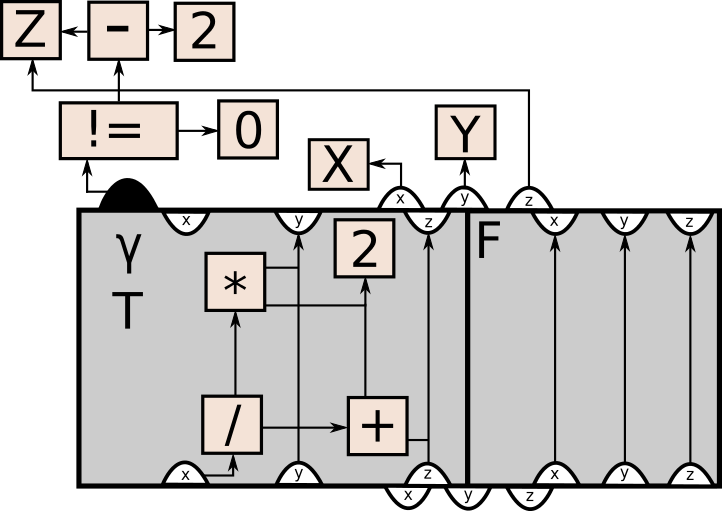
\includegraphics[width=\textwidth]{figures/simple_if_example}
	\end{minipage}
	\captionof{figure}{Example of an RVSDG subgraph equivalent to the C/C++
if-statement on the left.}
	\label{fig:simple_if}
\end{centering}

\subsubsection{Edges}

The RVSDG has two types of edges: data dependence edges and state dependence
edges. They represent data and state dependencies operations have to each other,
respectively. An example of data dependence edges are the operands used in an
addition is shown in \todo{Insert reference when above figure is
fixed.}Figure~\ref{}.

State dependence edges are used to preserve the semantics of the program when
the program has side-effecting operations. If there are no data dependencies
between operations, state dependence edges can give the needed order of
execution for the connected operations.

\subsubsection{Nodes}

The RVSDG has two kinds of nodes: simple nodes and complex nodes. Simple nodes
are used to represent primitive operations, such as addition and substraction.
The arity and order of inputs and outputs of any RVSDG node need to match its
operation.

One simple node of special interest for this report is the \applyNode . An
\applyNode~represents the call site of a function. The first input argument of
an \applyNode~is the function the \applyNode~invokes. The remaining inputs are
the arguments to this function. Likewise, its results are the results of the
invocation of its function. Order and arity of inputs and outputs need to match
the arguments and results of the funtion, respectively.

Complex nodes contain one or more RVSDG subgraphs, which is why they are also
referred to as \textit{regions}. Differing from the simple nodes with their
contained subgraph, complex nodes may besides the normal inputs and outputs also
have internal inputs and outputs. See Figure~\ref{} for how complex nodes route
external and internal inputs/outputs.

\todo[inline]{Insert empty figure of complex node, with text annotations
explaining internal/external inputs/outputs.}

The complex nodes of an RVSDG relevant for this report are as follows:

\begin{itemize}

\item \textbf{$\gamma$-nodes: N-way statements}

\textit{$\gamma$-nodes} represent conditional statements. Each $\gamma$-node has
a predicate as first input. All other edges passing as inputs to the
$\gamma$-node are edges its subregions depend upon. Each subregion represents
one case from the predicate. All subregions must have the same order and arity
of internal inputs and outputs, even if the subgraph in each region does not
depend on all of the internal outputs.

A $\gamma$-node is equivalent to a \textit{switch-case} without fall-through in
C/C++. Each case of the switch statement corresponds to a subregion of the
$\gamma$-node. Hence, a simple \textit{if-statement} with no else-clause can be
represented by a $\gamma$-node with two subregions. The true subregion contains
the RVSDG subgraph that represents the body of the if-statement, whereas the
false subregion of the $\gamma$-node simply routes all inputs through. See
Figure~\ref{fig:simple_if} for an example of a $\gamma$-node.

\item \textbf{$\theta$-nodes: Tail-controlled loops}

\textit{$\theta$-nodes} represent tail controlled loops. As with
$\gamma$-nodes, its inputs (and outputs) are all the dependencies needed for the
RVSDG subgraph in its subregion.

The first time the operations of the node are executed, the external inputs are
mapped to the internal outputs. And likewise, the last iteration the operations
of the node are executed, the internal inputs are mapped to the external outputs
of the $\theta$-node.

However, inside the $\theta$-node there is an extra first internal input, which
is the predicate of the tail controlled loop. If this predicate evaluates to
true, the rest of the internal inputs of the $\theta$-node are mapped to their
corresponding internal outputs. This enables the iterative behaviour of an RVSDG
$\theta$-node. Thus, the operations represented by its contained RVSDG subgraph
can be executed as a tail-controlled loop.

A $\theta$-node is equivalent to a \textit{do-while} loop in C/C++, as shown in
Figure~\ref{fig:factorial_loop_ex}. See Listing~\ref{lst:factorial_loop_ex} for
the C/C++ code corresponding to the RVSDG depicted in
Figure~\ref{fig:factorial_loop_ex}.

\begin{centering}
	\noindent\begin{minipage}{\textwidth}
		\begin{CenteredBox}
		\begin{lstlisting}[style=global_customcpp]
unsigned int i = 0;
unsigned int r = 1;
do{
	i += 1;
	r *= i;
} while(i < n);
		\end{lstlisting}
		\end{CenteredBox}
	\end{minipage}
	\captionof{lstlisting}{C/C++ code corresponding to the RVSDG in
Figure~\ref{fig:factorial_loop_ex}.}
	\label{lst:factorial_loop_ex}
\end{centering}

Other loops than tail-controlled loops can be represented by combining complex
nodes. A \textit{for-loop} can be represented by putting a $\theta$-node inside
of the \textit{true} clause of a $\gamma$-node conaining no nodes in the
subregion representing the \textit{false} clause. This is equivalent to a
\textit{for-loop} if the $\gamma$-node and $\theta$-node have the same predicate
expression.

\todo[inline]{In figure: Remove Lambda! Make smaller!}

\begin{figure}[H]
	\centering
	\includegraphics[width=\textwidth]{figures/iterative_factorial_ex}
	\caption{An RVSDG representing the C/C++ program code in
Listing~\ref{lst:factorial_loop_ex}.}
	\label{fig:factorial_loop_ex}
\end{figure}

\item \textbf{$\lambda$-nodes: Functions}

\textit{$\lambda$-nodes} represent functions. They contain an RVSDG subgraph
representing the body of a function. The internal inputs of a $\lambda$-nodes
represent the results of the function the $\lambda$-node represents in the
RVSDG. Respectively, its internal outputs represent the arguments of the
function. While $\lambda$-nodes don't have any external inputs, their external
output are what give the \applyNode s their first input, enabling them to invoke
the function represented by the $\lambda$-node.

The arity and order of a $\lambda$-node's internal inputs and outputs must match
the arity and order of the external inputs and outputs of all connected
\applyNode s.

Hence, when an \applyNode~connected with a $\lambda$-node is executed, the
external inputs of the \applyNode~are mapped to the internal outputs of the
$\lambda$-node, and likewise the external outputs are mapped internal inputs of
the two, respectively.

Figure~\ref{fig:iter_fib_phi} and Listings~\ref{lst:iter_fib_phi} illustrate the
workings of $\lambda$-nodes by depicting an RVSDG and the equivalent C/C++ code
for an iterative fibonacci function.

\todo[inline]{Add examples (listing + figure) mentioned in above paragraph!!!}

\item \textbf{$\phi$-regions: Recursive environments}

\textit{$\phi$-regions} represent recursive environments. They contain at least
one recursive $\lambda$-node. Like the $\lambda$-node, they have no external
inputs. However, the internal outputs of the $\phi$-region represent the links
utilized by the \applyNode s contained within to connect with the respective
$\lambda$-nodes also contained within the same $\phi$-region.

The internal inputs of a $\phi$-region receive the function invocation links
from the $\lambda$-nodes contained within. The internal inputs map to the
external outputs, thus enabling \applyNode s outside of the recursive
environment to connect with the $\lambda$-nodes.

An RVSDG representing the recursive fibonacci function written in C/C++ in
Listing~\ref{lst:fib_phi}, illustrates the usage of a $\phi$-region in
Figure~\ref{fig:fib_phi}.

\begin{centering}
	\noindent\begin{minipage}{\textwidth}
		\begin{CenteredBox}
		\begin{lstlisting}[style=global_customcpp]
unsigned int fib(unsigned int n){
	if (n < 2){
		return n;
	}
	return fib(n-1) + fib(n-2);
}
		\end{lstlisting}
		\end{CenteredBox}
	\end{minipage}
	\captionof{lstlisting}{C/C++ code corresponding to the RVSDG in
Figure~\ref{fig:fib_phi}.}
	\label{lst:fib_phi}
\end{centering}

\begin{figure}[h!]
	\centering
	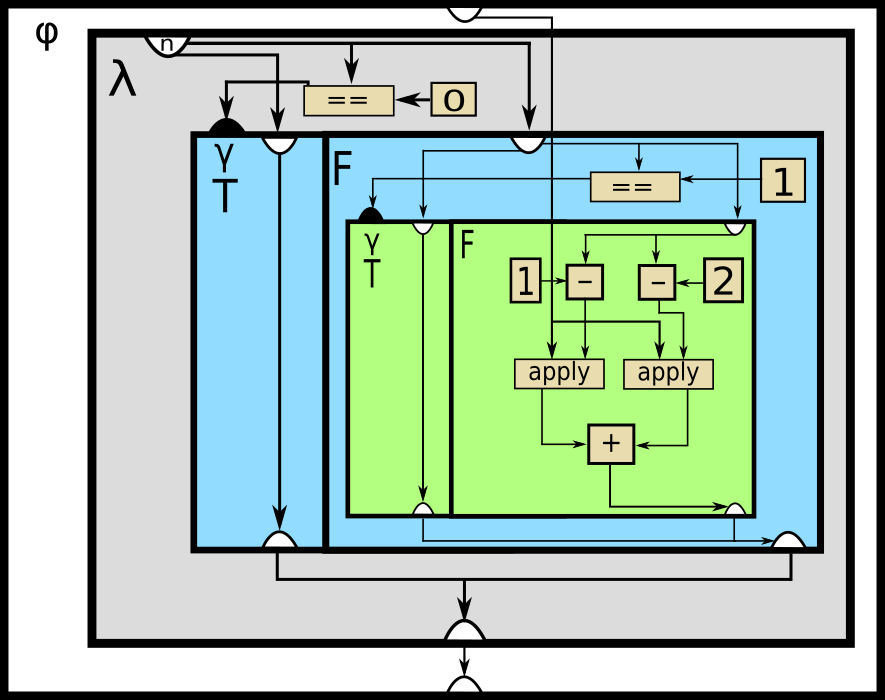
\includegraphics[width=\textwidth]{figures/recursive_fibonacci}
	\caption{An RVSDG representing the equivalent of the C/C++ code in
Listing~\ref{lst:fib_phi}. The RVSDG depicts a $\phi$-node containing a
$\lambda$-node representing a recursive version of a function producing the
\lstinline!n!th number in the Fibonacci series.}
	\label{fig:fib_phi}
\end{figure}

\end{itemize}
